\mysubsection{Lydia Friedrich}{Charaktere}

\begin{figure}[!htbp]%[htbp]
	\centering
		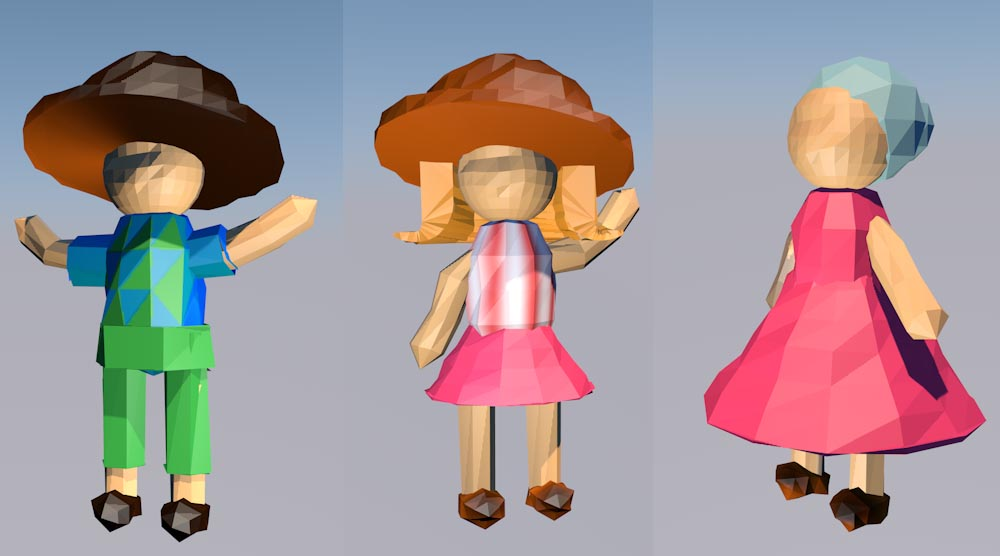
\includegraphics[width=0.9\textwidth]{images/Charaktere}
	\caption{Charaktermodelle}
	\label{fig:Frau1}
\end{figure}

Es gibt verschiedene Charaktere im Spiel:

\begin{itemize}
\item Wissenschaftler: Ist der Mentor des Spielers. Er ist aber gleichzeitig auch ein passiver Gegenspieler, da er der Verursacher des Weltenchaos ist. Er integriert den Spieler in seine eigene Welt und schickt ihn auf eine Heldenreise.
\item Spieler: Er ist der Protagonist und sieht die Welt mit seinen eigenen Augen. Er ist der Held des Spiels und hat die Möglichkeit die Welt des Wissenschaftlers zu retten.
\item Frau 1: Sie ist der erste NPC, mit dem der Spieler agiert. Sie trägt einen großen Hut und pinke Kleidung. Sie lebt schon seit ihrer Kindheit im Dorf und versteht sich mit allen sehr gut. Fremden gegenüber ist sie sehr offen und begrüßt den Spiele herzlich im Dorf. Animationen: Idle, Wave, Panic
\item Frau 2: Sie ist eine ältere Dame, die im Dorf lebt und dem Spieler das Gefühl gibt, nicht ganz alleine in der Welt zu sein. Gerne schaut sie aus ihrem kleinen Fenster und genießt das Leben im Dorf. Sie hat bereits graue Haare und trägt ein auffälliges pinkes Kleid. Sobald die Lichtmaschine wieder repariert ist, verlässt sie sofort ihr Haus. Animationen: Idle
\item Mann 1: Er ist der zweite NPC mit dem der Spieler interagiert. Durch den Vulkanausbruch steht sein Haus in Flammen und muss dringend gelöscht werden. Voller Panik wartet er auf Hilfe. Er trägt den dorftypischen Hut, ein blaues Oberteil und eine grüne Hose. Animationen: Idle, Wave, Panic
\item Mann 4: Er lebt mit seiner Familie in einem kleinen Haus am Rande des Dorfes. Seine Kinder spielen immer mit den Schafen. In letzter Zeit hat er Angst wenn die Kleinen draußen unterwegs sind. Jetzt, da das Licht wieder an ist jedoch nicht mehr. Auch er trägt das typische Dorfoutft. Animationen: Idle
\end{itemize}